%----------------------------------------------------------------------------------------
\chapter{Flow of dry water: Principles}
\label{ch:dry}
\section{Fluid particle and its acceleration}
Leaving hydrostatics, we now move on to flows.  To describe a
continuum we must now define a density and a velocity at every point
in the fluid. We have been doing this already, without much thought on
what we are actually doing. Let us now be somewhat finicky about
this.  

What we are doing here is setting up a \textit{field theory}. In
classical mechanics you have dealt with mechanics of single particle
and also several particles interacting with each other. The number of
degrees of freedom of such systems are finite, however larger.  To
specify a rigid body you have to specify its position (three numbers),
and orientation (three angles) giving rise to six numbers. As the
Newton's laws are second order in time, to specify an initial
condition you need to specify both position (that includes angles) and
velocities (that includes angular velocities). But to describe a
continuum medium you need an infinite number of degrees of
freedom. This is what a \textit{field} is.  One of the simplest
example is a density field, $\rho(\rr)$. A scalar that is a function
of position $\rr = (x,y,z)$.  
\marginnote{ The idea of a density field should give you pause. Mathematically we 
can define it by 
\begin{equation}
\rho(\rr) = \lim_{\Delta V \to 0}\frac{\Delta m}{\Delta V} 
\end{equation} 
Where $\Delta V$ is a small volume around the point $\rr$ and $\Delta
m$ is the mass in that volume.  But will this limit exist ?
Think about a glass of water.  What is the density at {\textit one mathematical point} ?
We know that the water is made out of molecules that are dancing
around. So if we really look at the mathematical point there may or
may not be a molecule at that point. So the density will be a highly
fluctuating quantity.  Even if we hit an atom, inside the atom there
are electrons and a nucleus. You know that the nucleus occupies a very
small position inside the atom and most of the atom is essentially
empty. So as we go to finer and finer scales we start seeing the
fundamentally discrete nature of matter. Hence to able to define a
density we need to work at scales much larger than the scale of
molecules. So the limit should be understood from a 
\textit{coarse-grained} view at a certain scale. 
How large should this scale be ? It should be large
enough to contain many molecules. }
Velocity is also a field in exactly the same sense. We do not ascribe velocity to a
mathematical point, but to a coarse-grained picture. A small volume in
the fluid contains many molecules with each molecule moving in a different direction.
 The typical speed of these molecules are set by the local temperature.
You may also know that the typical speed set by the temperature is of the
same order as the speed of sound in this medium. 
But the velocity field we want to take about is the mean velocity of a 
large number of molecules. 
For almost all cases we consider in these lectures, 
this velocity much smaller than the speed of sound in the medium. 
Imagine a larger number of molecules each moving with quite a high
speed in many different directions, but as far as their mean velocity is 
concerned the velocity of molecules moving in different directions cancel
each other so we land up with a velocity that is quite small compared to the
speed of individual molecules. This coarse-grained velocity itself is different
from one point in our medium to another. 

For the simplest fluid imaginable, other than velocity and density there is another 
property that we must consider, its temperature. We first want to consider the 
simplest case where both temperature and density of the fluid is a constant
but velocity is a function of space. This can be because the pressure is different in 
different parts of the fluid and also because of external forces acting on the fluid, e.g., gravity,
which is the only external force we consider at the moment.  What is the equation of motion 
of a small volume of fluid ? We had already deduced this in the previous lecture, \Eq{A1.2:motion},
\begin{equation}
\rho\frac{dV_{\alpha}}{dt} = \partial_{\beta}\sigma_{\alpha\beta}, \/,
\label{A2.1:dvdt}
\end{equation}
which is true for both fluid and deformable solids.
For fluid the stress tensor is given by, \Eq{A1.2:pressure}
$\sigma_{\alpha\beta} = -p \delta_{\alpha\beta}$, where $p$ is the pressure. 
Adding to this the gravity as an external force we eventually obtain
\begin{equation}
\rho\frac{dV_{\alpha}}{dt} = -\partial_{\alpha}p + \rho \ggg
\end{equation}
which we now write in vector form
\begin{equation}
\rho \frac{d\VV}{dt} = - \grad p + \rho \ggg
\label{A2.1:Lag}
\end{equation}
Remember this is the equation of a small parcel of fluid that itself moves in space.
In classical fluid mechanics nomenclature this small parcel of fluid is called a ``fluid particle''. 
Let me remind you how we derived \Eq{A2.1:dvdt}. The velocity $\VV$ is the rate at which 
the position of a particle and the RHS of \Eq{A2.1:dvdt} is calculated at its position. 
Let us assume that at time $t=0$, the same fluid particle was at the position $\rnot$. 
The position of the fluid particle as a function of time is then given by $\rr(t\mid\rnot,0)$
where the initial position is used to label the particle. The instantaneous velocity and position 
\begin{marginfigure}
\includegraphics{figures/LagPath.png}
\caption{A sketch of the trajectory of a Lagrangian 
particle. The tangent to this trajectory at any instant gives
the Lagrangian velocity as a function of time. This Lagrangian
velocity is also the Eulerian velocity at the position of the
Lagrangian particle.}
\label{fig:lagpath}
\end{marginfigure}
related by 
\begin{equation}
\frac{d}{dt} \rr(t \mid \rnot,0) = \VV(t\mid\rnot,0) \/,
\end{equation}
which implies
\begin{equation}
\rr(t\mid\rnot,0) = \rnot + \int_0^t\VV(s\mid\rnot,0) ds \/.
\label{A2.1:Ldisplacement}
\end{equation}
The displacement $\rr(t\mid\rnot,0)-\rnot$ is called the Lagrangian
displacement and $\VV(r\mid\rnot,0)$ the Lagrangian velocity. 
\marginnote{
A note for future references. In steady flows the Lagrangian 
particles do move along streamlines but not in general. So when
I am drawing a picture of Lagrangian trajectories they have nothing to
with the streamlines.  
}
Note that in our way of writing these equations, the velocity $\VV$ is not a function of 
position, it is not a \textit{field} in the usual sense of the word. It is rather a function of time. 
The space appears as a label that applies to the initial position of the fluid particle. 
So although we have derived an equation of motion for a fluid parcel
we have not got what we expected -- an equation of evolution of the
velocity field. Let me denote the velocity field at a point $\xx$ by
$\vv(\xx,t)$. In fluid dynamics the velocity field is typically called
\textit{Eulerian velocity}. 

Let us now revisit the acceleration term on the LHS of  \Eq{A2.1:dvdt}. 
\begin{equation}
\frac{d}{dt} \VV(t\mid\rnot,0) = 
\lim_{\Delta t\to 0}
\frac{
{\color{red}\VV(t+\Delta t\mid\rnot,0)} -
{\color{blue} \VV(t\mid\rnot,0)}
}
{\Delta t}
\label{A2.1:euler1}
\end{equation}
The {\color{blue} second term} in the numerator on the RHS of \Eq{A2.1:euler1} is
related to the velocity field as follows
\begin{equation}
\VV(t\mid\rnot,0)= \vv\left[\rr(t\mid\rnot,0),t\right] 
\label{A2.1:euler2}
\end{equation}
%-------------
\begin{marginfigure}
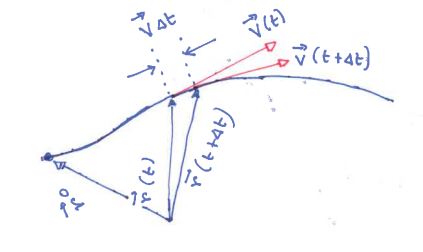
\includegraphics{figures/Drdt.png}
\caption{The difference between the Lagrangian velocity of the same
  Lagrangian particle at two different times is same as the difference
is Eulerian velocity at two different space locations -- the two
different positions of the Lagrangian particle at two different times.}
\label{fig:Drdt}
\end{marginfigure}
%---------------
where $\rr$ is the Lagrangian displacement given in
\Eq{A2.1:Ldisplacement}. 
In a small interval of time $t$ to $t+\Delta t$ the fluid parcel moves a
distance 
\begin{equation}
\Delta\rr \equiv \VV(t\mid \rnot,0)\Delta t =
\vv(\rr,t) \Delta t\/.
\label{A2.1:dr}
\end{equation}
 The {\color{red}first term}
on the numerator on the RHS of \Eq{A2.1:euler1} is then given by 
\begin{equation}
\VV(t+\Delta t\mid\rnot,0) = \vv(\rr+\Delta \rr,t+\Delta t) 
\label{A2.1:euler3}
\end{equation}
Substituting \Eq{A2.1:euler3} and \Eq{A2.1:euler2} in \Eq{A2.1:euler1}
and using \Eq{A2.1:dr} we obtain
\begin{equation}
\frac{d}{dt} \VV(t\mid\rnot,0) =
 \lim_{\Delta t\to0}
\frac{
{\color{red}\vv(\rr+\Delta \rr,t+\Delta t)} -
{\color{blue} \vv(\rr,t)}
}
{\Delta t}
\label{A2.1:euler4}
\end{equation}
\begin{fullwidth}
Now let us Taylor expand the first term in the numerator of
\Eq{A2.1:euler4} in a multi-variable Taylor series
\begin{eqnarray}
\vv(\rr+\Delta \rr,t+\Delta t)=& 
\vv(x+\Delta x,y+\Delta y, z+\Delta z,
t+\Delta t) \nonumber \\
&=\vv(\rr,t) + (\partial_x\vv)\Delta x + 
(\partial_y\vv)\Delta y +
(\partial_z\vv)\Delta z +
(\partial_t\vv)\Delta t  \nonumber \\   
&= \vv(\rr,t) +  \left[(\partial_x\vv)v_x + 
(\partial_y\vv)v_y +
(\partial_z\vv)v_z +
(\partial_t\vv) \right]\Delta t 
\label{A2.1:euler5}
\end{eqnarray}
where the last equality follows from \Eq{A2.1:dr}.
\end{fullwidth}
Compactifying the notation we can write \Eq{A2.1:euler5}
as
\begin{equation}
\vv(\rr+\Delta \rr,t+\Delta t) - \vv(\rr,t) = (\partial_t \vv+ \vv\cdot\grad\vv)\Delta t
\end{equation}
Substituting this back in \Eq{A2.1:euler4} we get
\begin{equation}
\frac{d}{dt} \VV(t\mid\rnot,0) = \partial_t \vv + \vv\cdot\grad\vv
\end{equation}
where the derivatives on the RHS are calculated at $\xx=\rr$ given by
\Eq{A2.1:Ldisplacement}. 
Putting the acceleration back in \Eq{A2.1:Lag} we obtain
\begin{equation}
\boxed{
 \partial_t \vv + \vv\cdot\grad\vv  = -\frac{\grad p}{\rho} + \ggg \/.
}
\label{A2.1:Euler}
\end{equation}
Allow me to remind you that we have assumed that the density $\rho$ is
a constant. The \Eq{A2.1:Euler} is the celebrated Euler equation. As you
can see, this is a partial differential equation which is first order
in space and time. To solve this we must specify boundary conditions. 
\marginnote{
{\bf Notation}\\
Often we use a single symbol for the material derivative
\begin{equation}
D_t \equiv \partial_t + \vv\cdot\grad
\end{equation}
}
The other property of this equation that you should note is that it is
\textit{non-linear} -- the second term on the LHS of this
equation. This term is also called the \textit{advective derivative}
of velocity. Both the beauty and the complexity of  fluid mechanics
owes its origin to this term. 
\marginnote{
You have learned the usual way of using vector identities to prove
\begin{equation}
\vv\cdot\grad\vv  = (\curl\vv)\times \vv + \frac{1}{2}\grad(\vv\cdot\vv)
\nonumber
\end{equation}
To show you the power of tensors, let me do it using what we have
learned so far. Using the Levi-civita tensor the first term on the RHS can be written as:
\begin{eqnarray}
&\epsilon_{\mu\alpha\nu}\epsilon_{\alpha\beta\gamma}(\partial_{\beta}v_{\gamma})v_{\nu}
\nonumber\\
&={\color{red}-\epsilon_{\alpha\mu\nu}}\epsilon_{\alpha\beta\gamma}(\ldots) \nonumber\\
&=-{\color{red}(\delta_{\mu\beta}\delta_{\nu\gamma}-\delta_{\mu\gamma}\delta_{\nu\beta})}(\ldots)
  \nonumber\\
=&-\delta_{\mu\beta}\delta_{\nu\gamma}
  (\partial_{\beta}v_{\gamma})v_{\nu} +
  \delta_{\mu\gamma}\delta_{\nu\beta}(\partial_{\beta}v_{\gamma})v_{\nu}
  \nonumber\\
=&- (\partial_{\mu}v_{\gamma})v_{\gamma} +
   (\partial_{\nu}v_{\mu})v_{\nu} \nonumber \\
=&  \vv\cdot\grad\vv - \frac{1}{2}\grad v^2
\end{eqnarray}
}
There is one crucial physical phenomenon that we have ignored so far in
this lecture, that is viscosity. We know from experience that viscous
forces exists.  If I stir my coffee with a spoon and then stop the
stirring, the flow slows down and eventually stops. This is because the
layers close to the boundary slows down because of ``friction''
between the coffee and the cup. The inner layers of the fluid slows
down because of the``friction'' between the outer layers and the
inner layers.  We shall spend quite a large fraction of these lectures
studying the effects of viscosity has on flows. The only exception is
this lecture and the next. 

In the ancient nomenclature the fluid that obeys the Euler equation is
called \textit{ideal} fluid.  There is nothing ``ideal'' about such a
fluid. Scientists have a tendency to take a word from everyday
language and then to ascribe special meaning to it -- a meaning may seem
to be an abuse of the word. The word ``ideal'' does not mean something
that normal fluid should aspire to be, it really means a hypothetical
fluid. Let me give you a more familiar example. 
You know the \textit{ideal} gas laws, although there are, in practice, no
ideal gases.  An ideal gas will remain a gas even when frozen to
zero-degree Kelvin. There is no such gas. But real gases behave close
enough  to ideal gases over a certain region of their phase-diagram. 
The gas laws themselves are not hypothetical they are results of
experiments. No flow can be described by the Euler equation, but in
some special cases certain quantities calculated from the Euler
equation may be a good approximation to those quantities in real
flows. This statement may seem too abstract at the moment. We shall
make it more precise near the end of this course. Following Feynman~\cite{Feynman77},
who himself borrowed the name from John Von Neuman, we shall call
\Eq{A2.1:Euler} the equation for flow of dry water. A more mundane but
accurate name is to call such flows \textit{inviscid flows}. 

\section{Bernoulli's equation}

As the gravity can also be written as the gradient of a potential we
can write \Eq{A2.1:Euler} as
\begin{equation}
 \partial_t \vv + \vv\cdot\grad\vv  = -\grad\left\{ \frac{p}{\rho} -\Psi\right\} \/.
\label{A2.1:E1}
\end{equation}
remembering that $\rho$ is a constant. 
Using the following vector identity
\begin{equation}
\vv\cdot\grad\vv  = (\curl\vv)\times \vv+
\frac{1}{2}\grad(\vv\cdot\vv) \/,
\label{A2.1:vdotv}
\end{equation} 
we can write \Eq{A2.1:E1} as 
\begin{equation}
 \partial_t \vv + (\curl\vv)\times \vv  = -\grad\left\{ \frac{p}{\rho}
   +\Psi + \frac{1}{2}v^2\right\} \/.
\label{A2.1:E2}
\end{equation}
\marginnote{
{\bf Statics, steady flow and statistically steady flow}:\\
In the last chapter, we studied hydrostatics, where $\vv=0$. Now we
consider the cases where fluid actually flows, but it does not change
with time $\partial_t \vv = 0$, although $\vv$ is a function of
space. Can this truly happen ? Consider for example a flow in a
pipe. If the pipe is not too big and the flow not too fast then you
shall find that the velocity of water in the pipe is a constant with
time. Although the velocity is different depending on how far you are
from the walls of the pipe -- at the wall the velocity is zero. But
this is true only when the pressure difference across the pipe is a
constant.  This you can manage by attaching the inlet of the pipe to a
water tank with is so large that within the time of your experiment
the height of the water in the tank does not change by any appreciable
amount. Again, it depends on length and time scales -- how large the tank is and how long your
experiment runs. 

Much later while considering turbulent
flow we shall consider \textit{statistically} steady flows, in which
case the flow velocity is not a constant but fluctuates a lot,
nevertheless its statistics (mean, and all the higher moments) does
not change with time. 
}
Now consider steady flows, $\partial_t \vv = 0$ and take a dot product
of both sides of \Eq{A2.1:E2} with the vector $\vv$ to obtain:
\begin{equation}
 \vv\cdot\grad\left\{ \frac{p}{\rho}
   +\Psi + \frac{1}{2}v^2\right\} = 0 \/.
\label{A2.1:bern}
\end{equation}
This is a remarkable result.  To appreciate this first consider what
the dot produce means. As the flow is steady, at every point there is
a constant velocity. I can think of a line, the tangent to which at
every point gives the velocity at that point. Along such a line the
quantity inside the curly braces in \Eq{A2.1:bern} is zero ! 
Such lines are called \textit{streamlines}. 

The statement \Eq{A2.1:bern} essentially is a statement of conservation of
energy. Consider a fluid parcel of volume $\delta V$ in a steady
flow. Given its initial position it will move along the streamline
that passes through that position. If we assume that energy is
conserved -- which is not the case as in practice viscous effects will
make the particle loose energy -- then the energy of this fluid parcel
will be constant as it moves along a the streamline. The energy is
precisely given by 
\begin{equation}
p\delta V + \delta V\rho \Psi + \frac{1}{2}\rho \delta V v^2\/.
\nonumber
\end{equation}
Here the first term comes from the work done due to pressure, the
second due to gravity and the last is the contribution from the
kinetic energy. A more detailed version of this derivation can be
found elsewhere, e.g.,  in Feynman~\cite{Feynman77}.

Now that we have arrived at the conservation of energy I shall now
postpone a longer discussion of the Bernoulli's equation and talk
about conservation laws in general for a moment. 

\section{Conservation Laws}

I have stated many times that the laws of hydrodynamics are a
particular example in a more general field, the theory of fields. 
 Let me start the discussion on conservation laws in a more general 
and more abstract spirit. 

Consider a system with large number of particles.
Let us assume that each of these particles interact with every other
particle. But all the interactions conserve certain quantities. For
example they conserve the number of particles. This mean that under
the interaction the particles may collide with each other but two of
them are not allowed to merge together. Or one of them is not allowed
to suddenly break up into two. 
 So we reach a conservation law
applicable to the whole volume:
\begin{gcon}
Total number of particles in the volume $V$ is a constant.  
\end{gcon}
%-------------
\begin{marginfigure}
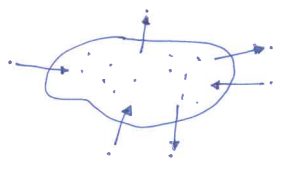
\includegraphics{figures/jj.png}
\caption{Particles moving in and out of a fixed volume in space.}
\label{fig:jj}
\end{marginfigure}
%---------------
If we consider any sub-volume  then the conservation law 
as written above is not true any more.  Because particle can enter or
leave this volume. But we can modify the conservation law in a minor
way to take care of this by saying
\begin{lcon}
Total number of particles in any sub-volume $\delta V$ plus the number
of particles that enter minus the number of particles that leaves is a
constant.  
\end{lcon}
Now we try to write a very similar law, instead of particles we
consider a continuum with a density $\rho$. Instead of number of
particles begin conserved we state that the total mass in the volume
$V$ must be conserved. A mathematical statement of this will be
\begin{equation}
\int_V dV \rho(\rr) = \text{constant} \/,
\end{equation}
or, in other words
\begin{equation}
\partial_t\int_V dV \rho(\rr) = 0 \/\quad.
\label{A2.1:gmass}
\end{equation}
This is the global conservation law, which applies to the whole
universe\footnote{Actually this statement is not completely
  true. According to the laws of nature as we know today mass can
  disappear to be replaced by energy. As a concrete example an
  electron and positron can annihilate each other to give rise to
  light. But if we add the energy to the mass conservation law then we
  are correct again.  In these lectures we shall stay away from both
  special and general relativity, hence mass itself is conserved. }.
But a local conservation law also holds:
\begin{equation}
\int_{\delta V} dV \rho(\rr) + 
\left(\parbox{2cm}{mass that enters $\delta V$}\right)- 
\left(\parbox{2cm}{mass that leaves $\delta V$}\right)
= \text{constant} \/,
\end{equation} 
which implies:
\begin{equation}
\partial_t\int_{\delta V} dV \rho(\rr) + 
\left(\parbox{2cm}{rate at which  mass enters $\delta V$}\right)
- \left(\parbox{2cm}{rate at which  mass leaves $\delta V$}\right) = 0 \/,
\label{A2.1:lmass}
\end{equation} 
Clearly mass must enter or leave the volume $\delta V$ through its
surface. So the second and third term on the LHS of \Eq{A2.1:lmass}
are surface terms.  They become clearer if we define a flux of
matter, $\JJ$. The flux is a vector, such that the amount of matter
that passes through a surface-element $\nhat dS$ in unit time is given by
$\JJ\cdot\nhat dS$. 
%-------------
\begin{marginfigure}
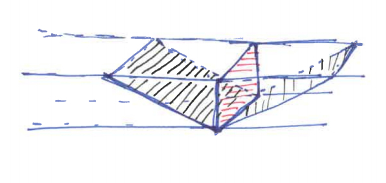
\includegraphics{figures/flux.png}
\caption{The flux of a quantity through a surface $\nhat dS$ is given by
the product of the flux vector $\JJ\cdot\nhat dS$. All the three
surfaces sketched above have the same flux. }
\label{fig:flux}
\end{marginfigure}
%---------------
Clearly
\begin{equation}
\left(\parbox{2cm}{rate at which  mass enters $\delta V$}\right) - 
\left(\parbox{2cm}{rate at which  mass leaves $\delta V$}\right)
= \oint_{S}\JJ\cdot\nhat dS \/,
\end{equation}
where the surface $S$ is a closed surface that bounds the volume
$\delta V$. 
Putting everything together we obtain
\begin{equation}
\partial_t \int_{\delta V} dV \rho(\rr)  = - \oint_{S}\JJ\cdot\nhat dS
\end{equation}
%-------------
\begin{marginfigure}
\includegraphics{figures/Jds.png}
\caption{The flux of through the surface which encloses a volume
is an integral over the surface. }
\label{fig:flux}
\end{marginfigure}
%---------------
Now we apply Gauss's theorem to the RHS of this equation to obtain
\begin{equation}
\partial_t \int_{\delta V} dV \rho(\rr)  = - \int_{\delta V}\dive \JJ dV
\end{equation}
Let us consider a volume $\delta V$ which itself does not change with
time. In that case, the time derivative on the LHS can be moved inside
the integral. Furthermore, this is true for any volume $\delta V$,
hence we obtain
\begin{equation}
\boxed{
\partial_t \rho + \dive \JJ = 0 \/.}
\label{A2.1:conservation}
\end{equation}
A wonderfully general relation that applies to any conserved
``density'' and its ``flux''. For example, in electrodynamics,
electrical charge is a conserved density variable, in that case the
vector $\JJ$ is the electrical current density.

The way it is written down now, \Eq{A2.1:conservation} is not of much
use to fluid mechanics; we do not know what the flux $\JJ$ is. But
what can move mass ? Mass can move only of there is a flow. The flux
of mass is then $\JJ = \rho\vv$. Substituting this in
\eq{A2.1:conservation} we get
\begin{equation}
\boxed{
\partial_t \rho + \dive (\rho\vv) = 0 \/.}
\label{A2.1:cont}
\end{equation}
This is one of the central equations of fluid mechanics. 
It is known as the \textit{continuity equation}. 
It is merely a statement of conservation of mass.  So far in this chapter we have
assumed that the density is a constant. But \eq{A2.1:cont} is more
general, it is true irrespective of whether density is constant or
not. 

If we apply \eq{A2.1:cont} to flows where the density is indeed a
constant, for example for water under most engineering and geophysical
situations, we obtain
\begin{equation}
\dive \vv = 0 \/.
\label{A2.1:incom}
\end{equation}
A fluid that obeys this, i.e., a fluid whose density is a constant, is
called an incompressible fluid. We shall sometime call
\eq{A2.1:incom} as the \textit{incompressibility constraint}.

\begin{Exercise}
\label{Ex3}
\Question
\label{prb3.1}
{\bf Vorticity equation}\\
Starting from \Eq{A2.1:E2} show that the Euler equation can also be
written in the form
\begin{equation}
\partial_t \oo + \curl (\oo\times\vv) = 0 \/.
\label{A2.1:vort}
\end{equation}
where $\oo=\curl\vv$. 
\Question
\label{prb3.2}
{\bf Incompressibility} 
\begin{enumerate}
\item  Show that for incompressible flows, $\dive \vv = 0$, in the absence of
any external force including gravity, the pressure and
velocity are related by the following relation
\begin{equation}
\lap p = - \dive(\vv\cdot\grad\vv)\/.
\end{equation} 
\item Can we have sound waves in a truly incompressible fluid ?
\end{enumerate}
\end{Exercise}
